% ============================================================
%  Chapter 3 — Method
% ============================================================
\chapter{Method}
\label{ch:method}

The purpose of this chapter is to answer two questions: which model predicts the albedo
and the shading, and how CIAI trains it. We start with the physical model that underlies IID
(\secref{sec:physics}), because it fixes what the network must output. We then describe the
network architecture (\secref{sec:architecture}), and finally the CIAI training strategy
(\secref{sec:ciai}), which is the core of this thesis.


\section{Physical Model}
\label{sec:physics}

\subsection{The Standard IID Equation}

Under the Lambertian reflectance model and a white (achromatic) illuminant,
the intensity at a pixel $p$ in an image is:
\begin{equation}
  \mathbf{I}(p) = \mathbf{A}(p) \cdot S(p)
  \label{eq:iid}
\end{equation}
where $\mathbf{A}(p) \in [0,1]^3$ is the three-channel albedo (material
reflectance) and $S(p) \in \mathbb{R}_{>0}$ is a non-negative scalar shading
value. Shading describes the illumination arriving at the surface point after
geometry, visibility, and shadows have had their effect. Albedo describes the
fraction and colour of that light that the material diffusely reflects. The
camera observes the reflected result, not either factor in isolation.

Under the assumption of a grey (achromatic) illuminant, $S$ is a scalar and the
product in \eqnref{eq:iid} is a simple element-wise multiplication: each colour
channel of $\mathbf{I}$ is scaled by the same amount.
This makes the colour of each pixel determined entirely by $\mathbf{A}$.

\subsection{Why Achromatic Shading Fails with Coloured Light}

When the illuminant has colour, the scaling is no longer the same across channels.
A red lamp makes the $R$ channel brighter relative to $G$ and $B$.
A correct model would encode this in the shading, but scalar shading cannot express
different scalings per channel.
What actually happens in practice is that the model absorbs the channel imbalance
into the albedo, because the albedo is the only RGB term in the equation.
The predicted albedo therefore reflects the combined colour of the surface
\emph{and} the illuminant, rather than just the surface.

\figref{fig:formulation} demonstrates that this is a limitation of the
representation, not a particular network. Even when the scalar model is given
the luminance of the true RGB shading, dividing the image by that scalar can
change brightness but cannot remove the lamp's hue.

\begin{figure}[t!]
  \centering
  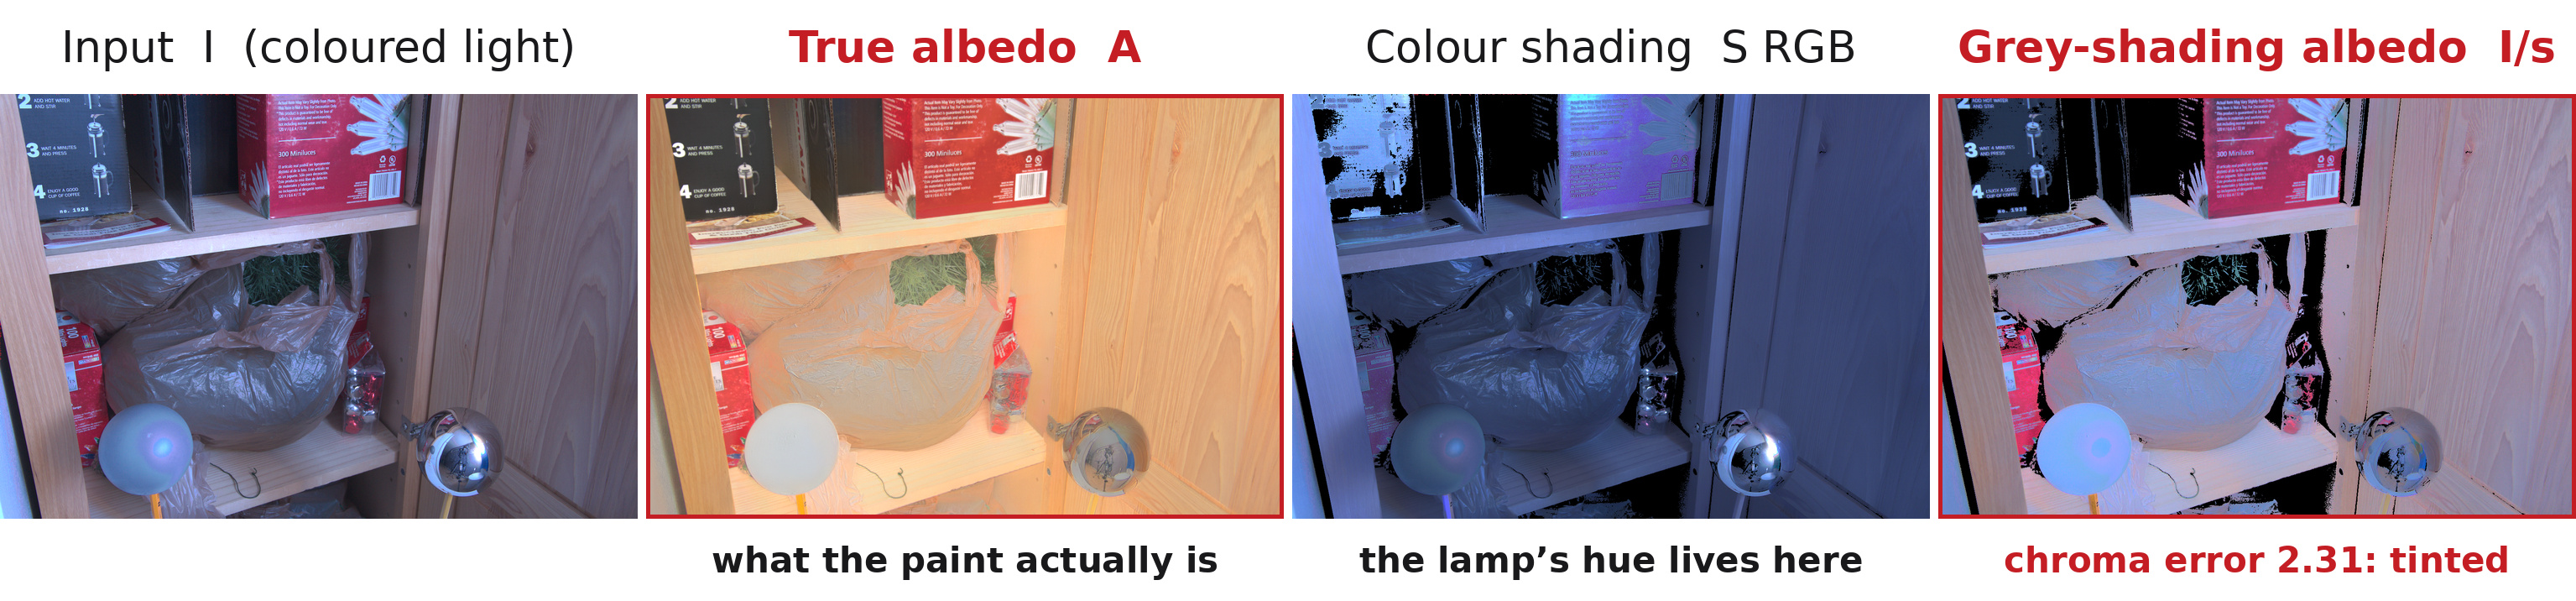
\includegraphics[width=\textwidth]{images/formulation/formulation.jpg}
  \caption[Why scalar shading leaks illuminant colour into albedo.]{%
    Why scalar shading must leak illuminant colour into albedo. From left: a
    warm-lit MID frame; pseudo-ground-truth albedo; the RGB shading implied by
    the data; and the albedo recovered with the luminance of that true shading.
    Even with the luminance of the true shading, the scalar construction gives a visibly
    tinted albedo, because a scalar can change brightness but not hue. Its mean chroma
    error, the per-pixel distance to the pseudo-ground truth in $(R/G, B/G)$, is $2.31$,
    against $0.22$ when the shading has three channels; that small remainder comes from
    clipped pixels.
  }
  \label{fig:formulation}
\end{figure}

To model coloured illumination correctly, the shading must therefore be a
three-channel (RGB) quantity $\mathbf{S}_d(p) \in \mathbb{R}_{>0}^3$, so each
colour channel can be scaled independently.
The model additionally keeps an explicit non-diffuse term for the light that the
Lambertian product cannot represent (specular highlights, visible light sources,
clipped pixels), giving the full decomposition:
\begin{equation}
  \mathbf{I}(p) = \mathbf{A}(p) \odot \mathbf{S}_d(p) + \mathbf{R}(p)
  \label{eq:iid_color}
\end{equation}
where $\odot$ is element-wise multiplication, $\mathbf{S}_d$ is the coloured
\emph{diffuse} shading, and $\mathbf{R} \geq 0$ is the non-diffuse residual.
The model predicts $\mathbf{A}$ and $\mathbf{S}_d$ with two network heads and derives
the residual \emph{analytically} as
$\mathbf{R} = \bigl(\mathbf{I} - \mathbf{A} \odot \mathbf{S}_d\bigr)_{+}$,
so the reconstruction $\mathbf{A} \odot \mathbf{S}_d + \mathbf{R}$ matches the
input by construction wherever the diffuse product does not overshoot it.

A three-channel shading solves the representation problem but not the
\emph{ambiguity} problem: single-image supervision cannot say how much of a hue
belongs to the albedo and how much to the shading colour, and the standard
ground-truth datasets (including Hypersim) supervise shading only up to this
ambiguity.
Paired observations can narrow this ambiguity. If the albedo is required to be
identical across two images of a scene whose illuminant colours differ, any part of the
illuminant colour that \emph{differs} between the two frames can no longer sit in the
albedo. Two limits follow directly, and both turn out to matter. A colour common to both
frames (a constant tint) satisfies the constraint and is left unresolved; and the
constraint can only remove colour differences that the training pairs actually contain.
\secref{sec:ciai} defines the losses and \secref{sec:colour_axis} measures how much of
this the real pairs deliver.

\subsection{The Shading Parameterisation}

A practical challenge in predicting shading is that it can take any positive
value, which is an unbounded output range; worse, its distribution in
real scenes is heavily skewed.
Specular surfaces and bright light sources produce very large shading values,
so linear shading concentrates almost all pixels in a narrow band near zero
with a long tail (\figref{fig:inverse_shading}): a regression loss on this
representation is dominated by a few extreme pixels while the mid-range
values that carry the shadow structure receive almost no gradient.
Working in the logarithmic domain balances the distribution but still has no
well-defined range for a network output.
Following the inverse-shading parameterisation of \mycitetext{careaga23ordinal},
which was introduced to solve exactly this conditioning problem,
the network predicts a bounded quantity
$\boldsymbol{\pi}(p) = 1 / \bigl(\mathbf{S}_d(p) + 1\bigr) \in (0, 1)$
per channel using a sigmoid activation, and the shading is recovered by
inverting this mapping:
\begin{equation}
  \mathbf{S}_d(p) = \frac{1 - \boldsymbol{\pi}(p)}{\boldsymbol{\pi}(p)}
  \label{eq:uninvert}
\end{equation}
The prediction is clamped to
$\boldsymbol{\pi} \in [5 \times 10^{-3},\, 1 - 10^{-4}]$, which bounds the
recovered shading to $\mathbf{S}_d \in [10^{-4},\, 199]$, providing enough headroom to
represent bright high-dynamic-range illumination while keeping the division
numerically safe.
The inversion is differentiable, so gradients flow through it during training.
Losses that supervise the shading pattern are computed on $\boldsymbol{\pi}$
(bounded, well-conditioned), while physics losses that need the actual light
intensity (reconstruction, the residual) use the linear $\mathbf{S}_d$.

% fig:inverse_shading — regenerated from our own Hypersim data by
% tests/viz/build_inverse_shading_figure.py. The panels are raster (they are images); the
% three distributions are drawn here as pgfplots so they are vector, sharp at any zoom, and
% set in the document's own fonts. Data: chapters/data/shading_hist_*.dat
\begin{figure}[t!]
  \centering
  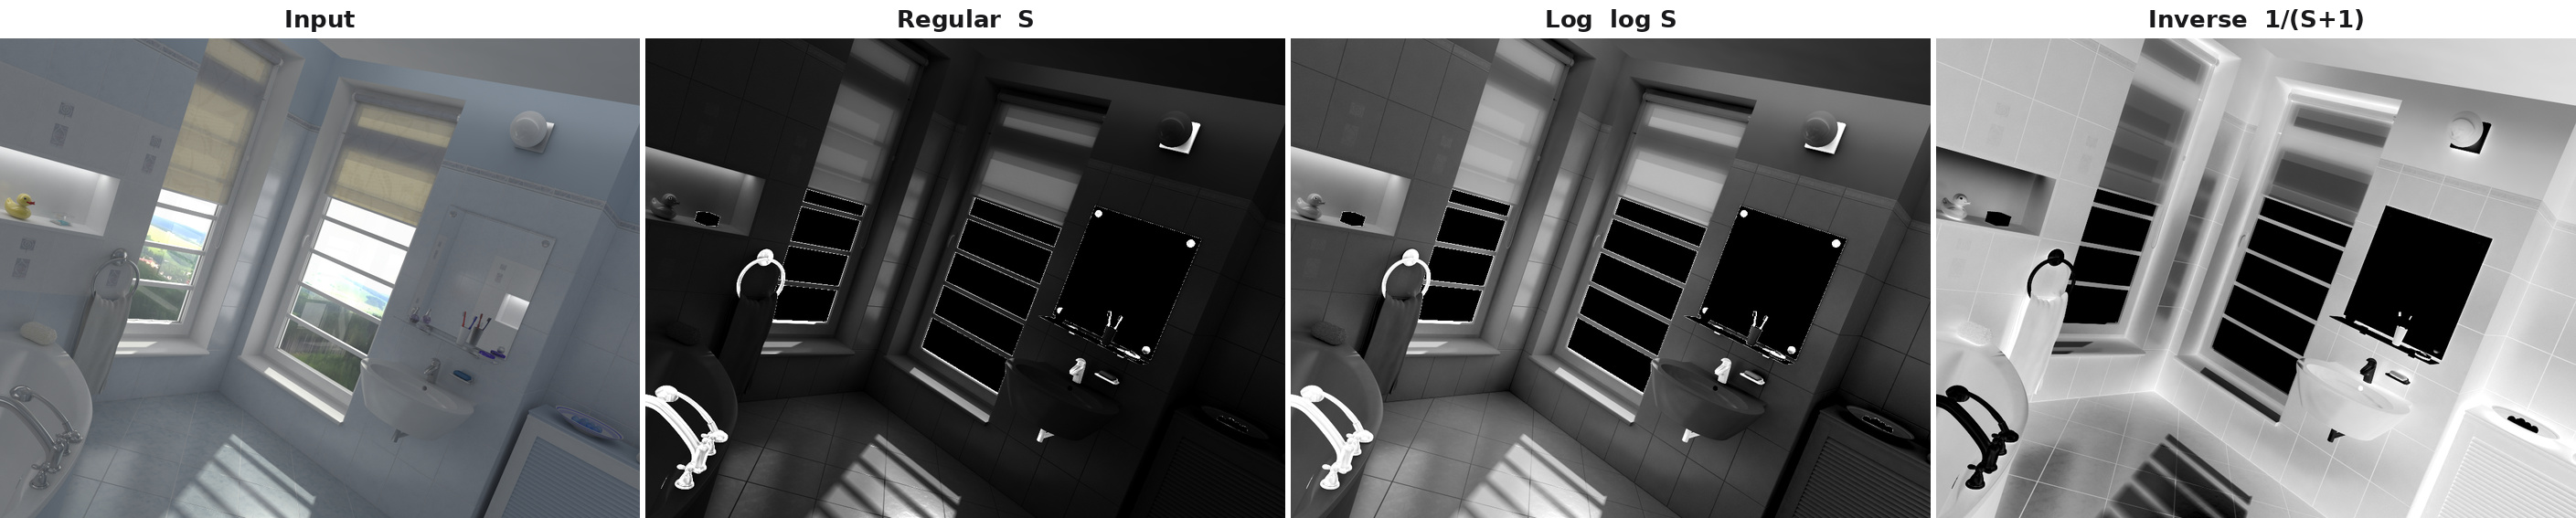
\includegraphics[width=\textwidth]{images/inverse_shading/panels.jpg}\\[6pt]
  \pgfplotsset{
    shadinghist/.style={
      width=0.35\textwidth, height=3.6cm,
      ybar, bar width=1.1pt,
      ymin=0, ymax=1.10,
      axis lines=left,
      axis line style={gray!55},
      tick label style={font=\scriptsize},
      xlabel style={font=\scriptsize, yshift=2pt},
      ylabel style={font=\scriptsize},
      ytick=\empty,
      minor tick num=0,
      xtick align=outside,
      grid=none,
      title style={font=\scriptsize, yshift=-2pt},
      every axis plot/.append style={
        fill=blue!50!cyan, draw=none},
    }}
  \begin{tikzpicture}
    \begin{axis}[shadinghist, xlabel={$S$ \, (linear)}, ylabel={density},
                 xmin=-0.15, xmax=5.4, xtick={0,1,2,3,4,5},
                 title={Regular: mass collapses at $0$}]
      \addplot table[x=x, y=y] {chapters/data/shading_hist_regular.dat};
    \end{axis}
  \end{tikzpicture}\hfill
  \begin{tikzpicture}
    \begin{axis}[shadinghist, xlabel={$\log S$},
                 xmin=-1.75, xmax=1.8, xtick={-1.5,-0.5,0.5,1.5},
                 title={Log: balanced but unbounded}]
      \addplot table[x=x, y=y] {chapters/data/shading_hist_log.dat};
    \end{axis}
  \end{tikzpicture}\hfill
  \begin{tikzpicture}
    \begin{axis}[shadinghist, xlabel={$1/(S+1)$},
                 xmin=-0.03, xmax=1.03, xtick={0,0.25,0.5,0.75,1},
                 title={Inverse: spread across $[0,1]$}]
      \addplot table[x=x, y=y] {chapters/data/shading_hist_inverse.dat};
    \end{axis}
  \end{tikzpicture}
  \caption[Inverse-shading parameterisation and target distributions.]{%
    Why shading is regressed in the inverse domain. Shading is derived from Hypersim ground
    truth as $S = \mathbf{I} / \mathbf{A}$ and shown in three representations, with the
    distribution of its values beneath each.
    Linear shading is dominated by a small number of very bright pixels. It runs to
    $5.3$ on this frame, so almost all of the mass collapses into the first bin and a
    regressor spends its capacity on outliers.
    Log shading balances the distribution but has no bounded range, so it cannot be produced
    by a saturating output nonlinearity.
    Inverse shading, $1/(S+1)$, is confined to $[0,1]$ \emph{by construction} and spreads
    across it, which makes it a well-conditioned target for a sigmoid head: this is the
    representation our shading branch predicts (\secref{sec:physics}), following
    \mycitetext{careaga23ordinal}. The physics losses that need real light intensity operate
    on the linear $\mathbf{S}_d$ recovered from it.
  }
  \label{fig:inverse_shading}
\end{figure}



\section{Network Architecture}
\label{sec:architecture}

Our model is built on two components: a frozen DINOv2-Large visual encoder and a
DPT-style decoder with separate output heads for albedo and shading.

\subsection{DINOv2 Encoder}

The encoder is DINOv2-Large \mycite{oquab24dinov2}, a Vision Transformer (ViT)
with a patch size of 14 pixels and approximately 304 million parameters.
DINOv2 was trained with self-supervised learning on a large and diverse image
corpus, and it produces patch-level feature representations that capture
rich semantic and geometric information.

We use DINOv2 in a frozen state, meaning its weights are not updated during
IID training.
This is a deliberate design choice for two reasons.
First, DINOv2's representations are already very strong; fine-tuning them would
require careful learning rate scheduling and risks destroying useful features
learned during self-supervised pre-training.
Second, keeping the encoder frozen reduces GPU memory during training, which
allows us to use a larger batch size.

For an input image of size $H \times W$, DINOv2 divides it into $(H/14) \times (W/14)$
patches and produces a token embedding for each patch.
We extract the intermediate features from four roughly evenly-spaced transformer
blocks (blocks 5, 12, 18, and 24 of the 24-block ViT-L, the last of which is the
final block).
These multi-depth features capture information at different levels of abstraction:
earlier blocks retain more local texture and colour, while later blocks encode
semantic and structural information.
DINOv2 is trained to be invariant to strong photometric augmentation, so we expect its
patch tokens to change little with illumination: a shadowed and a lit patch of the same
material should map to similar tokens, which would help the model assign them the same
albedo. We did not test this property directly.

\subsection{DPT Decoder}

The Dense Prediction Transformer (DPT) decoder \mycite{ranftl21dpt} was designed
to reconstruct full-resolution feature maps from the patch tokens of a ViT.
The key idea is to re-assemble the patch tokens from each layer into a spatial
feature map, then fuse the maps from all layers through a series of convolutional
feature fusion blocks.
The fusion progressively upsamples the features to the input resolution,
combining coarse semantic information from deep layers with fine spatial details
from early layers.

We use a single DPT decoder that takes all four feature levels as input.
Each level is first \emph{reassembled}: the patch tokens are projected and
reshaped into a spatial feature map at a level-specific resolution.
The four maps are then merged by a chain of \emph{fusion} blocks, each of
which upsamples the coarser map, adds the next finer one, and refines the sum
with residual convolutions, so semantic context from deep blocks and spatial
precision from early blocks accumulate into one representation.
Because the ViT operates on $14 \times 14$ patches, even the finest token map
is far below pixel resolution; a lightweight convolutional \emph{detail stem}
therefore processes the raw input image in parallel and injects genuine
high-frequency edge information that the token path cannot carry.
The decoder output is a shared full-resolution feature map, which is fed to
two separate output heads.

\subsection{Output Heads}

The albedo head takes the DPT feature map, concatenates a full-resolution
\emph{RGB skip} (the gamma-encoded input image), and passes the result through
a small convolutional block followed by a sigmoid activation:
\begin{equation}
  \mathbf{A} = \sigma\Bigl(\text{Conv}\bigl(\mathbf{F}_{\text{DPT}},\,
               \mathbf{I}^{1/2.2}\bigr)\Bigr) \in [0, 1]^{H \times W \times 3}
  \label{eq:albedo_head}
\end{equation}
The sigmoid bounds the albedo to $[0,1]^3$, the correct range for a reflectance
value.
The RGB skip, together with the chroma-direction loss on albedo of
\secref{sec:losses}, forms what we call the \emph{colour path}. It is a design choice of this
model and not part of CIAI: the frozen semantic tokens do not seem to carry all of the
local, absolute colour needed for albedo, and without the skip the predicted albedo comes out visibly pale, with a
higher chroma error against the pseudo-ground truth (\secref{sec:ablation}); we did not probe the encoder directly, so the reason is a
hypothesis. The skip has a cost as well: it is a direct route by which the
\emph{illuminant} colour of the input can reach the albedo as a colour cast, which the
invariance loss must then counteract. The colour path is one of the two ablation axes in
\chapref{ch:experiments}.

The shading head applies its own convolutional block and sigmoid and outputs the
three-channel inverse shading:
\begin{equation}
  \boldsymbol{\pi} = \sigma\bigl(\text{Conv}(\mathbf{F}_{\text{DPT}})\bigr)
  \in (0, 1)^{H \times W \times 3}
  \label{eq:shading_head}
\end{equation}
The coloured diffuse shading $\mathbf{S}_d$ is recovered from $\boldsymbol{\pi}$
using \eqnref{eq:uninvert}, and the non-diffuse residual follows analytically:
\begin{equation}
  \mathbf{R} = \bigl(\mathbf{I} - \mathbf{A} \odot \mathbf{S}_d\bigr)_{+}
  \label{eq:residual}
\end{equation}
There is no third head: the residual costs no parameters, and the reconstruction
$\mathbf{A} \odot \mathbf{S}_d + \mathbf{R}$ is exact wherever the diffuse
product does not overshoot the image.

Both heads share the same DPT feature map as input.
This encourages the two predictions to be consistent with each other, since they
are both derived from the same underlying scene representation.

% fig:architecture — CRefNet-style pipeline for our model, with the supervised losses.
% Thumbnails: tests/viz/gen_arch_thumbs.py (data-only model), images/arch/*.png.
\begin{figure}[p]
  \centering
  \resizebox{\textwidth}{!}{%
  \begin{tikzpicture}[
      font=\sffamily, >=latex,
      thumb/.style={inner sep=0pt, draw=black!55, line width=0.4pt},
      blk/.style={draw=black!45, rounded corners=2pt, align=center, minimum height=15mm,
                  minimum width=12mm, line width=0.5pt, font=\small},
      dino/.style={blk, fill=teal!16, draw=teal!55, minimum height=30mm},
      dpt/.style={blk, fill=myblue!14, draw=myblue!55, minimum height=30mm},
      head/.style={blk, fill=orange!16, draw=orange!60},
      resid/.style={blk, fill=black!12, draw=black!50, minimum width=30mm},
      loss/.style={draw=red!55!black, circle, fill=red!7, inner sep=1pt, minimum size=8.5mm,
                   font=\footnotesize, text=red!60!black},
      io/.style={align=center, font=\small},
      dim/.style={font=\scriptsize\itshape, text=black!55, align=center},
      flow/.style={->, line width=0.8pt, black!70},
      lossflow/.style={->, line width=0.6pt, red!55!black},
      skipC/.style={->, line width=0.9pt, red!62!black, dashed},
    ]
    % rows: albedo (top, y=+11), trunk (mid, y=0), shading (bottom, y=-11)
    % ── encoder + decoder (mid row) ─────────────────────────────────
    \node[thumb] (imgT) at (0,0) {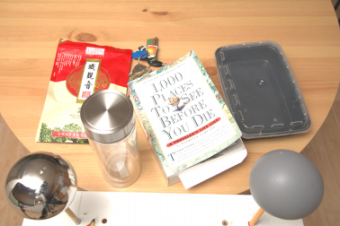
\includegraphics[width=19mm]{images/arch/input.png}};
    \node[io, above=0.5mm of imgT] {Input $\mathbf{I}$};
    \node[dino, right=9mm of imgT] (dino) {DINOv2-L/14\\[2pt]\emph{frozen}\\[2pt]{\scriptsize 4 stages, $\mathrm{d}{=}1024$}};
    \node[dim, above=0.4mm of dino] {material tokens};
    \node[dpt, right=10mm of dino] (dpt) {DPT\\decoder};
    \node[dim, below=0.5mm of dpt] {$768{\to}384{\to}192{\to}96{\to}64$};

    % ── heads (top / bottom rows) ───────────────────────────────────
    \node[head, above right=7mm and 12mm of dpt] (ah) {Albedo\\head};
    \node[head, below right=7mm and 12mm of dpt] (sh) {Shading\\head};

    % ── outputs + thumbnails ────────────────────────────────────────
    \node[io, right=8mm of ah] (Asym) {$\mathbf{A}\!\in\![0,1]^3$};
    \node[thumb, right=2.5mm of Asym] (albT) {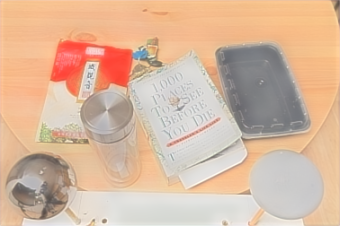
\includegraphics[width=15mm]{images/arch/albedo.png}};
    \node[io, right=8mm of sh] (Ssym) {$\boldsymbol{\pi}\!\in\!(0,1)^3$\\[1pt]$\mathbf{S}_d{=}\tfrac{1-\boldsymbol{\pi}}{\boldsymbol{\pi}}$};
    \node[thumb, right=2.5mm of Ssym] (shaT) {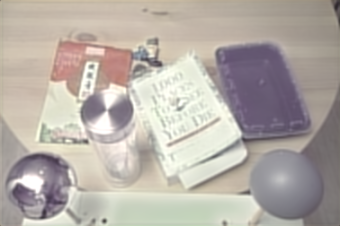
\includegraphics[width=15mm]{images/arch/shading.png}};

    % ── analytic residual: MUST sit downstream (right) of albT/shaT, since it is
    % computed FROM A and S_d, so the A->R and S_d->R arrows read left to right.
    % R shares the row of imgT/dino/dpt: x from albT.east, y from dpt.center via `let`.
    \path let \p1 = ([xshift=20mm]albT.east), \p2 = (dpt.center) in
      node[resid] (R) at (\x1,\y2)
      {$\mathbf{R}{=}(\mathbf{I}{-}\mathbf{A}{\odot}\mathbf{S}_d)_{+}$\\[1pt]{\scriptsize analytic; \emph{no head}}};
    % Residual thumbnail sits to R's RIGHT (not below), on the way to its loss, mirroring
    % how albT/shaT sit between their heads and their own loss nodes.
    \node[thumb, right=6mm of R] (resT) {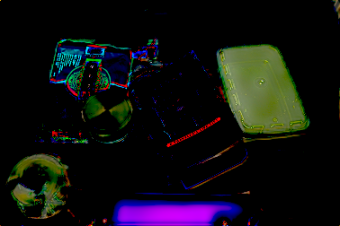
\includegraphics[width=13mm]{images/arch/residual.png}};

    % ── flows ───────────────────────────────────────────────────────
    \draw[flow] (imgT) -- (dino);
    \draw[flow] (dino) -- node[dim,above]{4 lvls} (dpt);
    \draw[flow] (dpt.east) -- ++(3mm,0) |- (ah.west);
    \draw[flow] (dpt.east) -- ++(3mm,0) |- (sh.west);
    \draw[flow] (ah) -- (Asym); \draw[flow] (Asym) -- (albT);
    \draw[flow] (sh) -- (Ssym); \draw[flow] (Ssym) -- (shaT);
    % A and S_d both feed R from the LEFT (upstream), arrowheads pointing right/down and
    % right/up INTO R — matches the left-to-right flow of the rest of the diagram.
    \draw[flow] (albT.south) -- ++(0,-4mm) -| (R.north);
    \draw[flow] (shaT.north) -- ++(0,4mm)  -| (R.south);

    % ── RGB skip: the only input skip actually enabled (shading has none;
    % rgb_shading.yaml sets shading_lum_skip=false, albedo_chroma_skip=false) ───────
    \draw[skipC] (imgT.north) |- ([yshift=7mm]ah.north) -| (ah.north)
      node[dim,pos=0.25,above,text=red!55!black]{RGB skip $\mathbf{I}^{1/2.2}$ (3\,ch, colour)};

    % ── SUPERVISED LOSSES (right column) ────────────────────────────
    \node[loss, right=10mm of albT] (la) {$\mathcal{L}_{\text{a}}$};
    \node[dim, right=0.5mm of la, text=red!55!black, align=left]
      {$+\,\mathcal{L}_{\text{msg-a}},\mathcal{L}_{\text{dssim}}$\\$+\,\mathcal{L}_{\text{chroma}},\mathcal{L}_{\text{mat}}$};
    \node[loss, right=10mm of shaT] (ls) {$\mathcal{L}_{\text{s}}$};
    \node[dim, right=0.5mm of ls, text=red!55!black, align=left]
      {$+\,\mathcal{L}_{\text{msg-s}},\mathcal{L}_{\text{sign}}$};
    % R.north = incoming A, R.south = incoming S_d (set above); R.east feeds the residual
    % thumbnail, which in turn feeds L_res — the same pattern albT->la and shaT->ls use.
    \node[loss, right=8mm of resT] (lr) {$\mathcal{L}_{\text{res}}$};
    \node[dim, above=0.3mm of lr, text=red!55!black]{sparsity $|\mathbf{R}|{\to}0$};

    \draw[lossflow] (albT) -- (la);
    \draw[lossflow] (shaT) -- (ls);
    \draw[flow] (R.east) -- (resT.west);
    \draw[lossflow] (resT.east) -- (lr);
    % CIAI acts on the albedo too (training-only; detailed in fig:ciai)
    \node[loss, above=4mm of la, draw=red!55!black, fill=red!7] (linv) {$\mathcal{L}_{\text{inv}}$};
    \node[dim, right=0.5mm of linv, text=red!55!black, align=left]{cross-illumination\\(\figref{fig:ciai})};
    \draw[lossflow, dashed] (albT.north) to[bend left=12] (linv.west);

    % ── legend (own row, below everything) ──────────────────────────
    \coordinate (legY) at ([yshift=-24mm]sh.south -| imgT.west);
    \begin{scope}[shift={(legY)}]
      \node[dino, minimum height=5mm, minimum width=7mm] (l1) {};
      \node[io, right=1.5mm of l1] (l1t){frozen encoder};
      \node[dpt, minimum height=5mm, minimum width=7mm, right=7mm of l1t] (l2) {};
      \node[io, right=1.5mm of l2] (l2t){DPT decoder \scriptsize(trained)};
      \node[head, minimum height=5mm, minimum width=7mm, right=7mm of l2t] (l3) {};
      \node[io, right=1.5mm of l3] (l3t){output head \scriptsize(trained)};
      \node[loss, minimum size=6mm, right=8mm of l3t] (l4) {};
      \node[io, right=1.5mm of l4] (l4t){loss};
      \draw[skipC] ([xshift=8mm]l4t.east) -- ++(6mm,0);
      \node[io, right=1mm of l4t, xshift=14mm] (sc){RGB skip};
    \end{scope}
  \end{tikzpicture}}
  \caption[Model architecture and supervision.]{%
    Model architecture and its supervision (\secref{sec:architecture}). The DINOv2-Large
    encoder (teal) is frozen; only the DPT decoder (blue) and the two output heads (amber),
    $18.5$M parameters, are trained. The albedo head also receives the input image through an
    RGB skip (the colour path); the shading head predicts the inverse shading
    $\boldsymbol{\pi}$, and the residual $\mathbf{R}$ is computed analytically, with no third
    head. Red nodes are the training losses on each output; $\mathcal{L}_{\text{inv}}$ acts
    across a pair at training time only (\figref{fig:ciai}). Thumbnails are outputs of our
    model on a MID test scene.
  }
  \label{fig:architecture}
\end{figure}



\section[Cross-Illumination Albedo Invariance (CIAI)]{Cross-Illumination Albedo\newline Invariance (CIAI)}
\label{sec:ciai}

\subsection{The Core Idea}

CIAI is a training strategy, not a change to the network.
It adds two loss terms that operate on \emph{pairs} of images of the same scene
photographed under different illumination. The design follows the Siamese pattern of
representation learning \mycite{chen21simsiam}: one network with shared weights processes
both views, and only positive pairs are used. Unlike a learned embedding, the quantity the
two views must share here is a dense physical map, the albedo.

Let $(\mathbf{I}_1, \mathbf{I}_2)$ be such a pair, where $\mathbf{I}_1$ and
$\mathbf{I}_2$ show the same scene under two different illuminations; on MID, two
different flash directions.
Let $\mathbf{A}_1 = \mathbf{A}(\mathbf{I}_1)$ and $\mathbf{A}_2 = \mathbf{A}(\mathbf{I}_2)$
be the albedos predicted by the model for each image, and let $S_1$ and $S_2$ be
the corresponding shadings.
\figref{fig:ciai} at the end of this section shows the complete mechanism, once
both losses below have been defined. \tabref{tab:ciai_glance} summarises each part of CIAI
as a goal, the idea behind it, and how it is implemented; the subsections below follow the
same order.

\begin{table}[t!]
  \caption[CIAI at a glance.]{%
    Each part of CIAI as a goal, the idea behind it, and its implementation.}
  \label{tab:ciai_glance}
  \centering
  \small
  \begin{tabular}{@{}>{\raggedright\arraybackslash}p{0.16\textwidth}>{\raggedright\arraybackslash}p{0.22\textwidth}>{\raggedright\arraybackslash}p{0.27\textwidth}>{\raggedright\arraybackslash}p{0.25\textwidth}@{}}
    \toprule
    Part & Goal & Idea & Implementation \\
    \midrule
    Invariance loss
      & The albedo must not change with the light.
      & The two frames show the same materials, so their albedos must agree.
      & Masked $\ell_1$ between $\mathbf{A}_1$ and $\mathbf{A}_2$ (\eqnref{eq:linv}). \\
    Explanation loss
      & Block the flat-albedo shortcut.
      & Where the albedo is shared, the image ratio equals the shading ratio.
      & Log luminance ratio of the shadings matches that of the images (\eqnref{eq:lexpl}). \\
    Validity mask
      & Train only on trustworthy pixels.
      & Clipped, specular and near-black pixels break the ratio.
      & Pixels between the 15th and 97th luminance percentile in both frames
        (\figref{fig:pair_mask}). \\
    Raw second frame
      & Keep the real colour change of the pair.
      & White balance would remove the illuminant colour.
      & First frame white-balanced and supervised, second frame raw (\figref{fig:wb_lanes}). \\
    Two-stage schedule
      & Anchor the albedo before asking for invariance.
      & On an unanchored model, invariance can be met by collapsing to grey.
      & Synthetic supervision to 19k iterations, then pairs added (\secref{sec:schedule}). \\
    \bottomrule
  \end{tabular}
\end{table}

\subsection{Invariance Loss}

The albedo must be the same for both images, because the physical material has not
changed.
We encode this as a masked $\ell_1$ loss:
\begin{equation}
  \mathcal{L}_{\text{inv}} =
  \frac{1}{|\Omega_v|} \sum_{p \in \Omega_v}
  \bigl\| \mathbf{A}_1(p) - \mathbf{A}_2(p) \bigr\|_1
  \label{eq:linv}
\end{equation}
where $\Omega_v \subset \Omega$ is the set of \emph{valid paired pixels}.
The validity mask matters in practice: MID frames are high-dynamic-range captures
that are clipped per frame, so a pixel can be saturated in one frame and not the
other, and deep shadows carry mostly sensor noise.
$\Omega_v$ keeps the pixels whose luminance lies between the 15th and 97th percentile in
both frames, with an absolute floor for near-black pixels, and drops the clipped pixels and
the brightest $3\%$ of the first frame that the supervised losses also ignore (roughly
$75\%$ of pixels survive, \figref{fig:pair_mask}). The invariance constraint is therefore
only applied where both observations are trustworthy.
This loss is zero only when the model predicts identical albedo for both images.
Minimising it pushes the albedo to be independent of whatever differs between the two
illuminations; it says nothing about a component the two frames share.

\begin{figure}[t!]
  \centering
  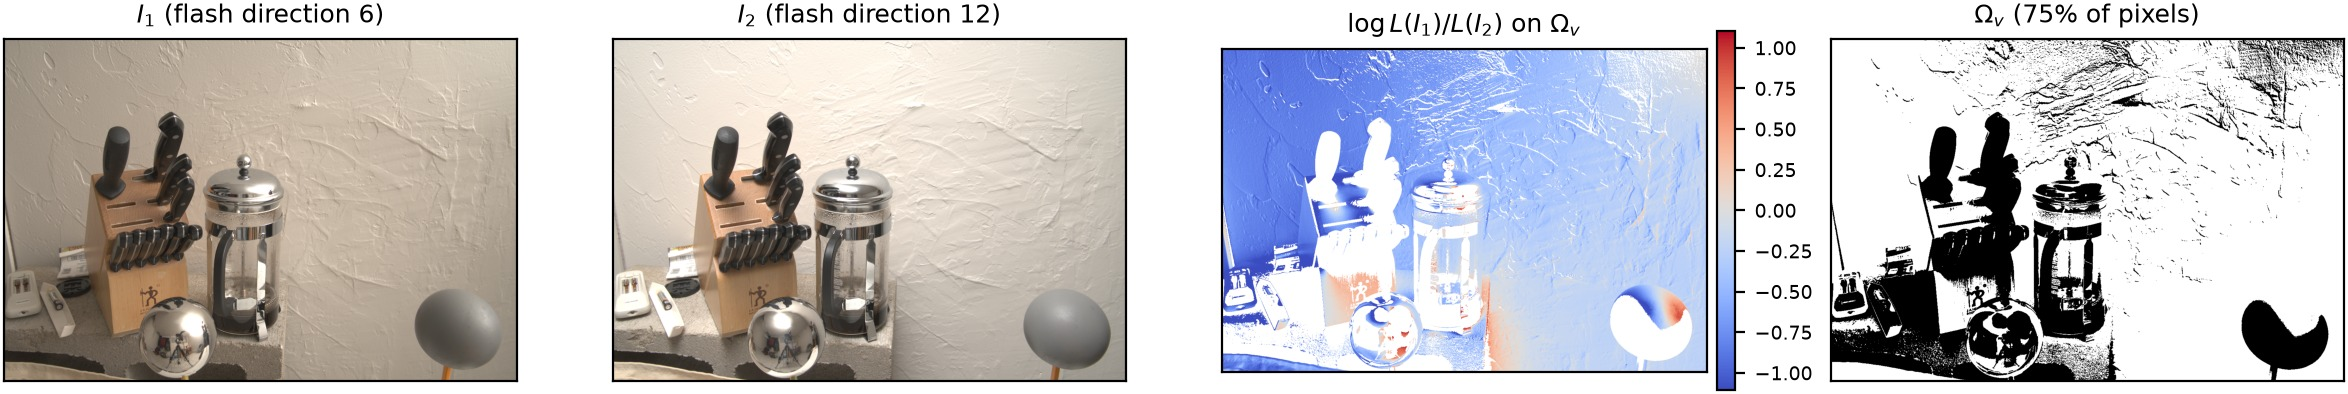
\includegraphics[width=\textwidth]{images/report/pair_mask.jpg}
  \caption[One CIAI training pair and its validity mask.]{%
    One CIAI training pair from MID, shown with a shared exposure. The third panel is the
    log luminance ratio of the two photographs, which $\mathcal{L}_{\text{expl}}$
    (\secref{sec:ciai}) asks the ratio of the two predicted shadings to match: blue where the
    second flash lights the surface more. The fourth panel is the validity mask $\Omega_v$,
    which keeps pixels between the 15th and 97th luminance percentile in both frames; here
    $75\%$ of the pixels survive. The specular highlights and the darkest shadows are
    removed, because their ratio says nothing about the diffuse shading.
  }
  \label{fig:pair_mask}
\end{figure}

\subsection{Explanation Loss}

The invariance loss alone is not enough.
A degenerate model could satisfy \eqnref{eq:linv} by predicting a flat, constant
albedo (the same grey image for every input).
To prevent this, we add a companion loss that requires the shading to \emph{explain}
the pixel-level difference between the two images.

Under the diffuse model $\mathbf{I} \approx \mathbf{A} \odot \mathbf{S}_d$, the
ratio of corresponding pixels in the two images equals the ratio of their
shadings wherever the albedo is shared:
\begin{equation}
  \frac{\mathbf{I}_1(p)}{\mathbf{I}_2(p)} = \frac{\mathbf{S}_{d,1}(p)}{\mathbf{S}_{d,2}(p)},
  \qquad \text{if } \mathbf{A}_1(p) = \mathbf{A}_2(p)
  \label{eq:explain_ratio}
\end{equation}
The material term cancels in the ideal diffuse image ratio, making the ratio a
useful lighting cue wherever registration is valid and non-diffuse effects are
small. Saturation, shadows, and specularities violate that idealisation; the
validity mask limits rather than eliminates those failures.
We enforce the constraint on the \emph{luminance} of both ratios, in the log
domain for numerical robustness:
\begin{equation}
  \mathcal{L}_{\text{expl}} =
  \frac{1}{|\Omega_v|} \sum_{p \in \Omega_v}
  \Bigl|
    \log\frac{L(\mathbf{I}_1(p)) + \varepsilon}{L(\mathbf{I}_2(p)) + \varepsilon}
  - \log\frac{L(\mathbf{S}_{d,1}(p)) + \varepsilon}{L(\mathbf{S}_{d,2}(p)) + \varepsilon}
  \Bigr|
  \label{eq:lexpl}
\end{equation}
where $L(\cdot)$ is the Rec.~601 luminance, $\varepsilon = 10^{-3}$, and
$\Omega_v$ is the same validity mask as in \eqnref{eq:linv}.
Using luminance makes this term supervise the achromatic \emph{intensity} change
between the frames, and only that. A purely chromatic change between the two frames
leaves both log-ratios in \eqnref{eq:lexpl} unchanged and contributes no gradient. Together
with $\mathcal{L}_{\text{inv}}$, which a colour shared by both albedos satisfies, nothing in
CIAI states where a change in illuminant \emph{colour} must go. This is why CIAI is
expected to help luminance more than colour (\secref{sec:colour_axis}).
This loss is zero only when the shading ratio matches the image ratio at every
valid pixel, which means the shading is absorbing the lighting difference rather
than the albedo.

\subsection{Raw Pairs and the Role of White Balance}
\label{sec:raw_pairs}

MID ships a grey probe in every frame, and the usual pre-processing white-balances each
frame by its own probe: the red and blue channels are rescaled so that the probe becomes
neutral, while the green channel, and with it the overall intensity, is left unchanged.
After this step the two frames of a pair differ in brightness and shadows exactly as
before, but their illuminant colours have been equalised.

For the second frame of the cross-illumination pair we skip this step (the
\texttt{mid\_raw\_color\_pair} flag). The first frame stays white-balanced, because it also
carries the supervised albedo loss and the pseudo-ground-truth albedo was derived from the
white-balanced stack. The second frame is left raw. The two frames of a pair therefore
differ in direction and intensity of the light, and also by the illuminant colour of the raw
frame relative to the neutral first frame, so $\mathcal{L}_{\text{inv}}$ is asked to be
invariant to that colour as well. \figref{fig:wb_lanes} shows one such pair.

The size of what is kept should not be overstated. MID's flash is white, and the colour
of a raw frame differs from neutral only through light bounced off coloured surfaces:
measured on the grey probes over the training pairs, the median chromaticity gap between the
two frames of a pair is $0.030$ (\secref{sec:colour_axis}). Keeping the pairs raw is therefore a choice that
preserves a small real colour signal, not a source of strong coloured-illuminant
supervision, and our ablations do not isolate its effect from the other components.

\begin{figure}[t!]
  \centering
  \begin{tikzpicture}[
      img/.style={inner sep=0pt, anchor=center},
      lab/.style={font=\footnotesize, align=center, text width=0.3\textwidth},
      loss/.style={font=\footnotesize, align=center, fill=white, inner sep=1.5pt},
      arr/.style={-latex, thick, black!70}]
    \node[img] (anc) at (0,0)    {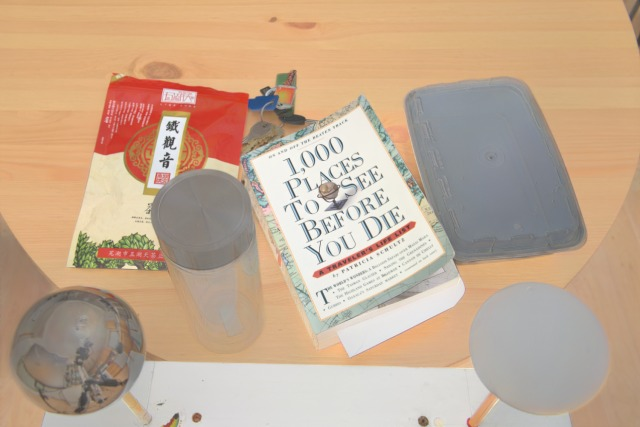
\includegraphics[width=0.29\textwidth]{images/wb/pair_anchor.jpg}};
    \node[img] (fa)  at (4.95,0) {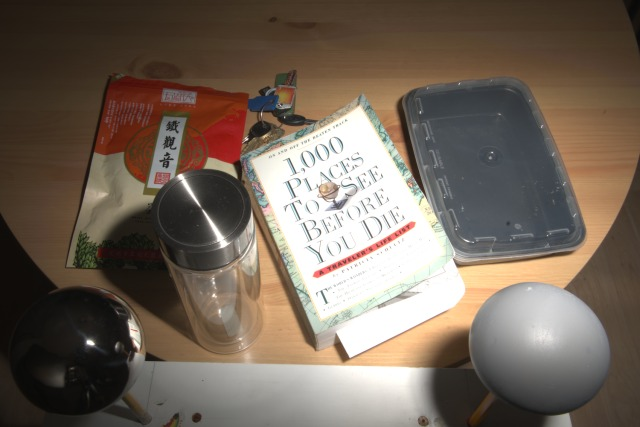
\includegraphics[width=0.29\textwidth]{images/wb/pair_frame_a_wb.jpg}};
    \node[img] (fb)  at (9.9,0)  {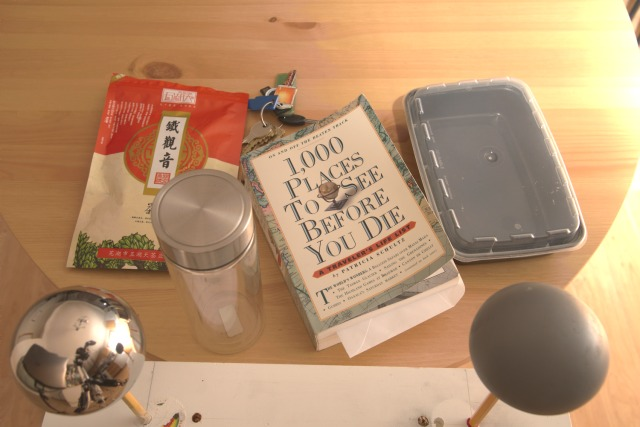
\includegraphics[width=0.29\textwidth]{images/wb/pair_frame_b_raw.jpg}};
    \node[lab, below=2pt of anc] {pseudo-ground-truth albedo\\(shared by all frames)};
    \node[lab, below=2pt of fa]  {frame $a$, \textbf{white-balanced}\\on its grey probe};
    \node[lab, below=2pt of fb]  {frame $b$, \textbf{raw}\\(keeps its illuminant colour)};
    \draw[arr, blue!70!black] ([yshift=4mm]fa.north) -- ++(0,0.5) -| node[loss, pos=0.25, text=blue!70!black]
      {supervised albedo loss} ([yshift=4mm]anc.north);
    \draw[arr, orange!80!black, latex-latex] ([yshift=4mm]fa.north east) -- ++(0,0.5) -| node[loss, pos=0.25, text=orange!80!black]
      {$\mathcal{L}_{\text{inv}}$, $\mathcal{L}_{\text{expl}}$} ([yshift=4mm]fb.north);
  \end{tikzpicture}
  \caption[How one CIAI training pair is pre-processed.]{%
    How one MID training pair is pre-processed (test scene, shown with one shared exposure).
    Frame $a$ is white-balanced, because it also carries the supervised loss against the
    white-balanced pseudo-ground-truth albedo. Frame $b$, a different flash direction, is left
    raw. The CIAI losses compare the two, so the albedo must ignore the change in light
    direction and intensity and also the colour of the raw frame. This example shows a large
    colour difference ($0.157$) to make it visible; the median over training pairs is $0.030$.
  }
  \label{fig:wb_lanes}
\end{figure}

% fig:ciai — CIAI training diagram, styled to match fig:architecture.
% Thumbnails from tests/viz/gen_ciai_thumbs.py (documents/thesis/images/arch/ciai_*.png).
\begin{figure}[t!]
  \centering
  \resizebox{0.96\textwidth}{!}{%
  \begin{tikzpicture}[
      font=\sffamily, >=latex,
      thumb/.style={inner sep=0pt, draw=black!55, line width=0.4pt},
      model/.style={draw=myblue!55, fill=myblue!12, rounded corners=2pt, align=center,
                    minimum width=17mm, minimum height=34mm, line width=0.5pt},
      loss/.style={draw=red!55!black, circle, fill=red!7, inner sep=1pt, minimum size=11mm,
                   font=\small, text=red!60!black},
      io/.style={align=center, font=\small},
      dim/.style={font=\scriptsize\itshape, text=black!55, align=center},
      flow/.style={->, line width=0.8pt, black!70},
    ]

    % ── the cross-illuminant input pair (real, pixel-aligned) ───────
    \node[thumb] (i1) {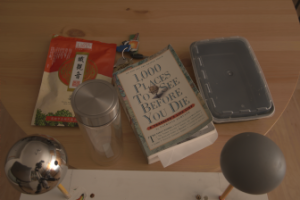
\includegraphics[width=20mm]{images/arch/ciai_I1.png}};
    \node[io, above=0.5mm of i1] {$\mathbf{I}_1$ \scriptsize(flash direction a)};
    \node[thumb, below=12mm of i1] (i2) {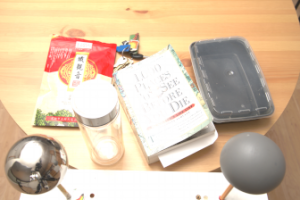
\includegraphics[width=20mm]{images/arch/ciai_I2.png}};
    \node[io, below=0.5mm of i2] {$\mathbf{I}_2$ \scriptsize(flash direction b)};
    \node[dim, below=4mm of i2] {same scene, pixel-aligned,\\raw (\emph{no} white balance)};

    % ── one model, shared weights, two forward passes ──────────────
    \node[model] (m) at ($(i1)!0.5!(i2) + (30mm,0)$) {Model\\[3pt]\emph{shared}\\\emph{weights}\\[3pt]{\scriptsize two forward}\\{\scriptsize passes}};

    % ── predicted albedos (should be identical) + shadings ─────────
    \node[thumb, right=16mm of m.east |- i1] (a1) {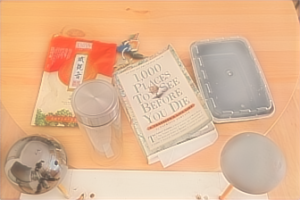
\includegraphics[width=15mm]{images/arch/ciai_A1.png}};
    \node[thumb, right=16mm of m.east |- i2] (a2) {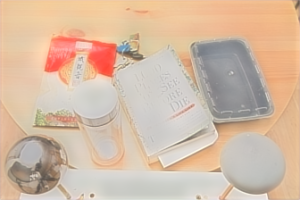
\includegraphics[width=15mm]{images/arch/ciai_A2.png}};
    \node[io, above=0.5mm of a1] {$\mathbf{A}_1$}; \node[io, below=0.5mm of a2] {$\mathbf{A}_2$};

    \node[thumb, right=26mm of a1] (s1) {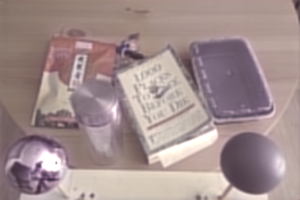
\includegraphics[width=15mm]{images/arch/ciai_S1.png}};
    \node[thumb, right=26mm of a2] (s2) {
\includegraphics[width=15mm]{images/arch/ciai_S2.png}};
    \node[io, above=0.5mm of s1] {$\mathbf{S}_{d,1}$}; \node[io, below=0.5mm of s2] {$\mathbf{S}_{d,2}$};

    % ── flows ──────────────────────────────────────────────────────
    \draw[flow] (i1.east) -- (m.west |- i1);
    \draw[flow] (i2.east) -- (m.west |- i2);
    \draw[flow] (m.east |- a1) -- (a1);
    \draw[flow] (m.east |- a2) -- (a2);
    \draw[flow] (a1.north) to[bend left=18] (s1.north west);
    \draw[flow] (a2.south) to[bend right=18] (s2.south west);

    % ── the two CIAI losses ────────────────────────────────────────
    \node[loss] (linv) at ($(a1)!0.5!(a2)$) {$\mathcal{L}_{\text{inv}}$};
    \draw[<->, red!55!black, line width=0.9pt] (a1.south) -- (linv);
    \draw[<->, red!55!black, line width=0.9pt] (a2.north) -- (linv);
    \node[dim, right=0.5mm of linv, text=red!55!black] {$\mathbf{A}_1\!=\!\mathbf{A}_2$\\\scriptsize (material only)};

    \node[loss] (lexp) at ($(s1)!0.5!(s2)$) {$\mathcal{L}_{\text{expl}}$};
    \draw[<->, red!55!black, line width=0.9pt] (s1.south) -- (lexp);
    \draw[<->, red!55!black, line width=0.9pt] (s2.north) -- (lexp);
    \node[dim, right=0.5mm of lexp, text=red!55!black, align=left]
      {$\dfrac{L(\mathbf{S}_{d,1})}{L(\mathbf{S}_{d,2})}\!=\!\dfrac{L(\mathbf{I}_1)}{L(\mathbf{I}_2)}$\\\scriptsize (shading explains the brightness change)};

  \end{tikzpicture}}
  \caption[Cross-Illumination Albedo Invariance during training.]{%
    Cross-Illumination Albedo Invariance (CIAI), applied only at training time. A
    pixel-aligned pair of the same MID scene under two flash directions is passed through
    the \emph{same} model (shared weights) in two forward passes. $\mathcal{L}_{\text{inv}}$
    ties the two predicted albedos $\mathbf{A}_1,\mathbf{A}_2$ together, and
    $\mathcal{L}_{\text{expl}}$ requires the luminance ratio of the two shadings
    $\mathbf{S}_{d,1},\mathbf{S}_{d,2}$ to match that of the two inputs. The second frame is kept
    raw (\secref{sec:raw_pairs}). Thumbnails are outputs of our model: the two albedos
    agree closely in luminance and less in colour, which is what the experiments of
    \chapref{ch:experiments} measure.
  }
  \label{fig:ciai}
\end{figure}

